\documentclass{standalone}
\usepackage{pgfplots}
\pgfplotsset{compat=1.18}
\usepgfplotslibrary{colorbrewer}
\pgfplotsset{cycle list/Set1-6}

\begin{document}

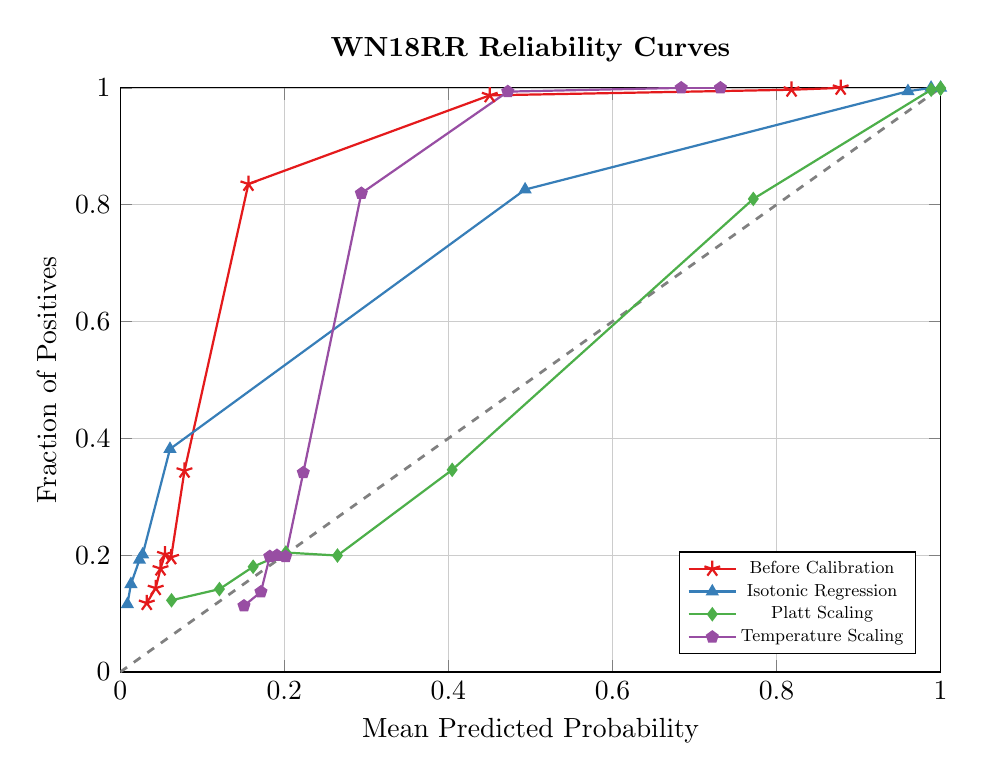
\begin{tikzpicture}
\begin{axis}[
    title={\textbf{WN18RR Reliability Curves}},
    xlabel={Mean Predicted Probability},
    ylabel={Fraction of Positives},
    xmin=0, xmax=1,
    ymin=0, ymax=1,
    xtick={0, 0.2, 0.4, 0.6, 0.8, 1.0},
    ytick={0, 0.2, 0.4, 0.6, 0.8, 1.0},
    legend pos= south east,
    legend style={nodes={scale=0.7, transform shape}, font=\small},
    grid=both,
    grid style={line width=.1pt, draw=gray!20},
    major grid style={line width=.2pt, draw=gray!40},
    width=12cm,
    height=9cm,
    cycle list name=Set1-6
]

% Perfectly Calibrated Line
\addplot [color=gray, dashed, line width=1pt, forget plot]
    coordinates {(0,0)(1,1)};

% Before Calibration (Baseline)
\addplot+[mark=star, thick, mark size=3pt] coordinates {
    (0.0323, 0.1180) (0.0432, 0.1435) (0.0491, 0.1770) (0.0545, 0.2013) (0.0620, 0.1962) (0.0783, 0.3445) (0.1562, 0.8355) (0.4504, 0.9872) (0.8183, 0.9968) (0.8782, 1.0000)
};
\addlegendentry{Before Calibration}

\addplot+[mark=triangle*, thick] coordinates {
    (0.0087, 0.1159) (0.0130, 0.1503) (0.0234, 0.1920) (0.0273, 0.2010) (0.0606, 0.3817) (0.4935, 0.8259) (0.9602, 0.9942) (0.9884, 1.0000) (1.0000, 1.0000)
};
\addlegendentry{Isotonic Regression}

\addplot+[mark=diamond*, thick] coordinates {
    (0.0625, 0.1228) (0.1209, 0.1419) (0.1620, 0.1802) (0.2019, 0.2045) (0.2648, 0.1994) (0.4046, 0.3461) (0.7717, 0.8099) (0.9885, 0.9968) (0.9999, 0.9984) (1.0000, 1.0000)
};
\addlegendentry{Platt Scaling}
\addplot+[mark=pentagon*, thick] coordinates {
    (0.1508, 0.1132) (0.1715, 0.1372) (0.1823, 0.1978) (0.1910, 0.1997) (0.2016, 0.1978) (0.2231, 0.3413) (0.2939, 0.8195) (0.4724, 0.9936) (0.6838, 1.0000) (0.7316, 1.0000)
};
\addlegendentry{Temperature Scaling}

\end{axis}
\end{tikzpicture}

\end{document}